\section{Architecture g�n�rale}

\subsection{Topologie}

\begin{center}
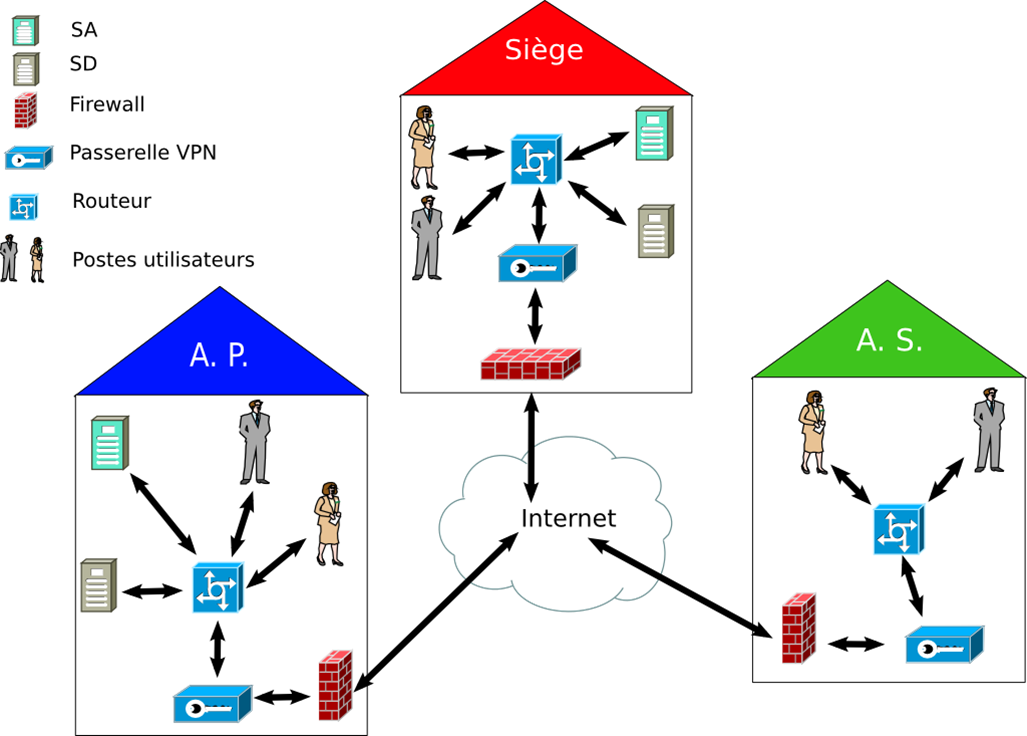
\includegraphics[width=10cm]{\PIXPATH/archi1}
\end{center}

Comme indiqu� sur le sch�ma ci-dessus, on installe un serveur de donn�es et un 
serveur applicatif au si�ge. Le serveur de donn�es du si�ge sert aussi de 
serveur de sauvegarde.
On implante un serveur applicatif et un serveur de donn�es par agence principale
tandis que les agences secondaires se content de se connecter aux agences 
principales.
Les agences et le si�ge sont tous reli�s entre eux par internet mais sont 
prot�g�s par un firewall. Cependant un r�seau VPN permet de virtualiser un 
r�seau priv� entre les agences et le si�ge.

\subsection{Implantation et Flux}

\begin{center}
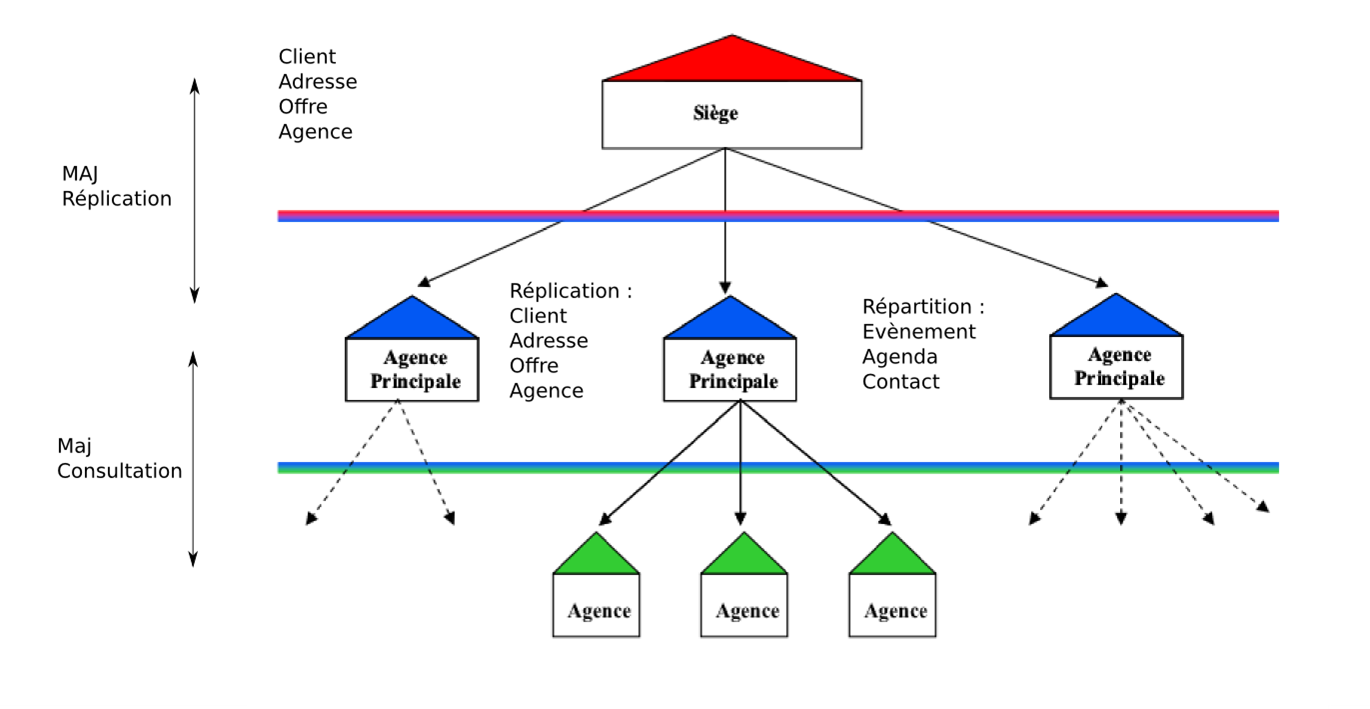
\includegraphics[width=10cm]{\PIXPATH/archi2}
\end{center}

Les applications Client, Adresse, Offre et Agence sont disponibles au si�ge. 
Ces m�mes applications sont r�pliqu�es dans les agences principales.
Les applications �v�nement, Agenda et Contact sont r�parties dans les agences
principales.

Au niveau des flux, entre le si�ge et les agences principales il y a des flux 
de Mise � Jour dans les deux sens et de r�plication du si�ge vers les agences.
Entre les agences principales et secondaires, on a des flux de mise � jour et 
de consultation dans les deux sens.